\documentclass[smallcondensed]{svjour3}     % onecolumn (standard format)
%\documentclass[smallextended]{svjour3}     % onecolumn (second format)
%\documentclass[twocolumn]{svjour3}         % twocolumn
%
\smartqed  % flush right qed marks, e.g. at end of proof
%
\usepackage{graphicx}
\usepackage{fix-cm}
%
% \usepackage{mathptmx}      % use Times fonts if available on your TeX system
%
% insert here the call for the packages your document requires
%\usepackage{latexsym}
% etc.
%
% please place your own definitions here and don't use \def but
% \newcommand{}{}
%
% Insert the name of "your journal" with
 \journalname{Swarm Intelligence}
%
\usepackage{makeidx} % allows for indexgeneration
\usepackage{graphicx}
\usepackage{multicol}
\usepackage{subfigure}
\usepackage{mathptmx} % use Times fonts if available on your TeX system
\usepackage{setspace}
\usepackage{natbib}
%
\begin{document}
\title{Implementing Continuous Flow of Information Using Centralized Communication for a Robotic Validation of the Attractive Field Model}
\titlerunning{Robotic Validation of the Attractive Field Model}
\author{Md Omar Faruque Sarker \and
Torbj{\o}rn S. Dahl %etc.
}
%\authorrunning{Short form of author list} % if too long for running head
\institute{
Cognitive Robotics Research Centre, University of Wales, Newport, UK\\
\email{Mdomarfaruque.Sarker $\mid$ Torbjorn.Dahl@newport.ac.uk}
}
%\date{Received: / / Accepted: / / }
% The correct dates will be entered by the editor
\maketitle
\begin{abstract}
Attractive field model is an interdisciplinary model of self-organization that proposes to solve the issue of division of labour or task allocation using a set of generic rules derived from the observation of ant, human and robotic social systems. These bottom-up rules can be used to model multi-robot task allocation problem in terms of attractive fields between robots and tasks. The concrete form of these rules provides  sufficient abstraction to accommodate different sensing and communication model.  By avoiding strong dependence on local interactions found in many existing approaches to  multi-robot task allocation, attractive field model  becomes flexible enough to achieve task allocation among multiple concurrent tasks through the presence of a system-wide continuous flow of information.  Unlike traditional swarm task-allocation which extensively relies upon local communication, our approach uses a centralized communication scheme to obtain continuous flow of information among variable number of  independent task-allocating robots. Our experimental  results validate the effectiveness of  using attractive filed model with a centralized communication scheme as a mechanism for self-organized multi-robot task allocation. Our experiments used 8 and 16 e-puck robots in 1m x 1m and 2m x 2m areas respectively.
%\keywords{Multi-robot system \and division of labour \and multi-robot task allocation}
%% \PACS{PACS code1 \and PACS code2 \and more}
%% \subclass{MSC code1 \and MSC code2 \and more}
\end{abstract}
%\addtolength{\parskip}{-3.5mm}
\section{Introduction}
\label{sec:intro}
%\vspace{2mm}
Multi-robot task allocation (MRTA) problem focuses on allocating appropriate tasks to appropriate robots dynamically considering the changes in task-requirements, team-performance and environment. This problem is analogous to the division of labour among individuals found in biological and human social systems. MRTA is a challenging research issue since there exist no central planner or coordinator in a distributed multi-robot team and robots have limited capabilities to sense, to communicate and to interact with a limited number of peers at a time. Due to large communication and computational overhead, traditional explicit task-allocation approaches, such as intentional cooperation \citep{Parker2008} and market-based bidding approach \citep{Dias+2006},  do not scale well to the large number of tasks and robots \citep{Lerman+2006}. On the other hand, existing self-organized approaches, such as emergent cooperation \cite{Kube+1993}, use of {\em adaptation rules} \citep{Liu+2007} are limited since they produce specific solutions to certain global tasks alone \citep{Gerkey+2004}.

As the part of the Engineering and Physical Sciences Research Council (UK) collaborative  research project, 'Defying the Rules: How Self-regulatory Systems Work', we have studied the behaviour of ants, humans and robots and formalized a set of necessary and sufficient requirements for self-organisation in social systems. These four requirements are: \textit{continuous flow of information}, \textit{concurrency}, \textit{learning} and \textit{forgetting} (which are explained later).  Primarily, these requirements facilitate the derivation of local control rules for regulating an individual's task-allocation behaviour in such a way that can develop self-organized division of labour in the entire group. However  unlike  most of the existing self-organized task-allocation approaches, these requirements do not assume the presence of any specific type of interaction or communication pattern of the group. 

The first requirement of  self-organization, i.e. continuous flow of information, demands that self-organised social systems must establish a flow of information over the period of time when self-organisation can be defined. The task information provides the basis on which the individuals self-organise by enabling them to perceive tasks and receive feedback on collective team performance.  Concurrence or the simultaneous presence of several task-options is the second requirement of  self-organization. This is necessary in order to meaningfully say that the system has organised into a recognisable structure. In task-allocation terms, the minimum requirement is a single task as well as the option of not performing any task. The third requirement of self-organization is the presence of different levels of sensitization among individuals towards different tasks. A system, where each robot has different levels of {\em sensitization} to the available tasks, can  embody a distinct organisation through differentiation. Finally, the last requirement of self-organization is to implement forgetting of tasks among individuals. In order to avoid saturation, forgetting mechanism reduces the sensitisation levels of individuals towards different tasks. This allows flexibility in the system as the individual preferences towards different tasks always keep changing over time. 

Based on the above requirements of self-organization we have developed a formal model of self-organized division of labour in social systems  named the {\em attractive field model} (AFM) \citep{Arcaute+2008}. We have selected the issue of division of labour since this is a well-understood problem in biological and human social systems. Now let us at first see how division of labour in ants, humans and robots can be explained in terms of the above four requirements. In an ant colony, we have assumed that division of labour is not genetically driven. Initially all ants are equal. It is not well-known how ants ``know'' or get information about tasks. But we know that they all interact directly and indirectly and perform tasks. The flow of information can take place in many different ways. Ants can get information through direct peer-to-peer, local or global broadcast and indirect pheromone communications. Thus each task can be treated as an attractive source, stimulating ants to go to it. Here the stimulus primarily depends on the distance. In case of sensitization or learning, an ant that has performed a task, it is assumed that it will be more likely that it will be attracted to do it again.  Concurrence of tasks  can also be achieved through spatial dependence of strength of stimulus. Some ants will be favoured to get information from multiple sources than others. When an ant does not do a task for relatively long time it is less probable that it will do that task again. This will lead to forgetting of their tasks gradually.  

Similarly, we can see that in human society people can get information about certain tasks or resources from various sources. Those who are located near the source of information are more likely to attend it. For example, trough the access to Internet, some people can get information quicker than others.  The background training, education or skill profile can be used to estimate the sensitization to do a task or use a resource. 

Similar to the above explanations, in a multi-robot system each robot can be modelled as an agent and each task can be modelled as a spatial location. Continuous flow of information is necessary to propagate the task-requirements to all robots. This flow of information can provide robots with necessary perception about task-requirements as well as the feedback about their collective performance. This flow of information can happen by global broadcast, local peer-to-peer interaction or even through stigmergy or a shared global memory. Our model does not assume any fixed communication set-up. Depending on a specific task performance, sensitization levels of robots for that task can be increased or decreased. Robots can have multiple options to select a task from a set of available tasks. If there is only a global task, e.g. in case of foraging task, random walking can be used as a no-task option. Thus using this abstract approach, we can effectively model the MRTA issue of a global task as well as multiple concurrent tasks in a multi-tasking environment. 

This article presents our works on the validation of the effectiveness of AFM in producing self-organized MRTA using a centralized communication scheme. The main contributions of this paper are: interpretation of AFM for a multi-robot system, implementation of the first requirement or the continuous flow of information and last, but not the least, validation of AFM in achieving self-organized MRTA in a fairly large multi-robot system. 

Rest of this article is organized as follows. Section~\ref{sec:afm} presents the interpretation of AFM for multi-robot systems.  Section~\ref{sec:rw} discusses related work and the correspondence of AFM with biological self-organization. Our centralized communication scheme is presented in Section~\ref{sec:comm}. Section~\ref{sec:expt} presents the design of our experiments including specific parameters and observables. Section~\ref{sec:res} discusses our experimental results from 8 and 16 robot experiemnts and section~\ref{sec:conc} draws conclusions..
%%%%%%%%%%%%%%%%%%%%%%%%%%%%%%%%%%%%%%%%%%%%%%%%%%%%%%%%%%%%%%%%%%%%%%%%%%%%%%%%%%%%
\section{The Attractive Field Model}
\label{sec:afm}
The AFM has been developed through a collaborative between the partners on the 'Defying the Rules: How Self-Regulated Social; Systems Work' project.  Experiments on ants colonies {\em Temnothorax albipennis} studied the collective performance of ants during brood-sorting and nest construction after emigration to a new site.  The model is also inspired by observational data from the self-organized development of the infrastructure of an {\em eco-village} by an open community of volunteers.  These studies helped us to formalize the a set of necessary and sufficient requirements for self-organisation in a social systems as discussed before. Below we discuss the generic framework of self-regulated division of labour under AFM and our interpretation of this framework for multi-robot systems.

Building on the requirements for self-organised social systems, AFM formalises these requirements in terms of the relationships between properties of individual agents and of the system as a whole \citep{Arcaute+2008}.  AFM is a bipartite network, i.e. there are two different types of nodes.  One set of nodes describes the sources of the attractive fields, the tasks, and the other set describes the agents.  Edges only exist between different types of nodes and they encode the strength of the attractive field as perceived by the agent.  There are no edges between agent nodes.  All communication is considered part of the attractive fields.  There is also a permanent field representing the {\em no-task} option of not working in any of the available tasks.  This option is modelled as a random walk.  
%%
\begin{figure}[htp]
%\begin{minipage}[t]{0.48\linewidth}
\centering
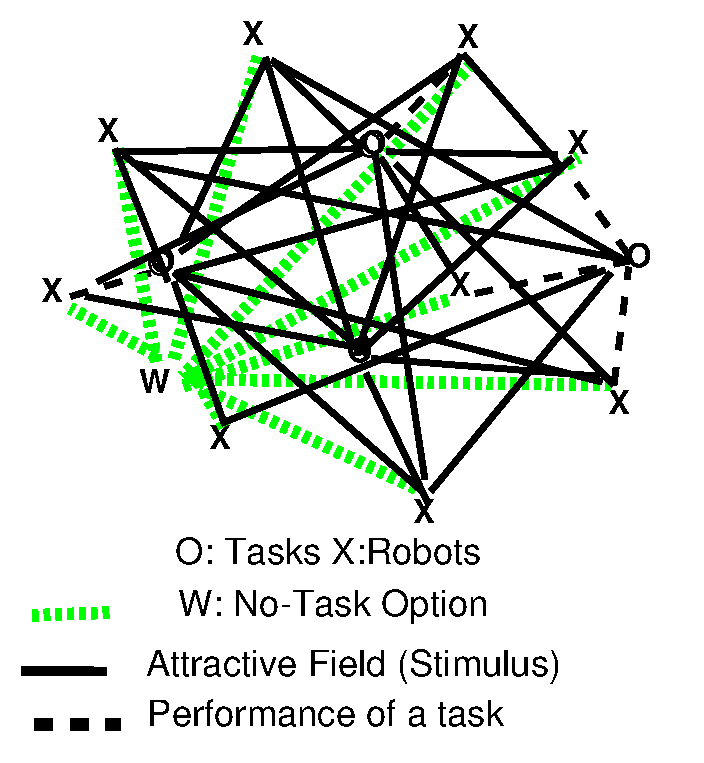
\includegraphics[height=4cm, angle=0]{./images/AFM-Diag3.eps}
%figure caption is below the figur
\caption{\small Attractive Filed Model (AFM)}
\label{fig:afm} % Give a unique label
%\end{minipage}
%\hspace{0.5cm}
%\begin{minipage}[t]{0.48\linewidth}
%\centering
%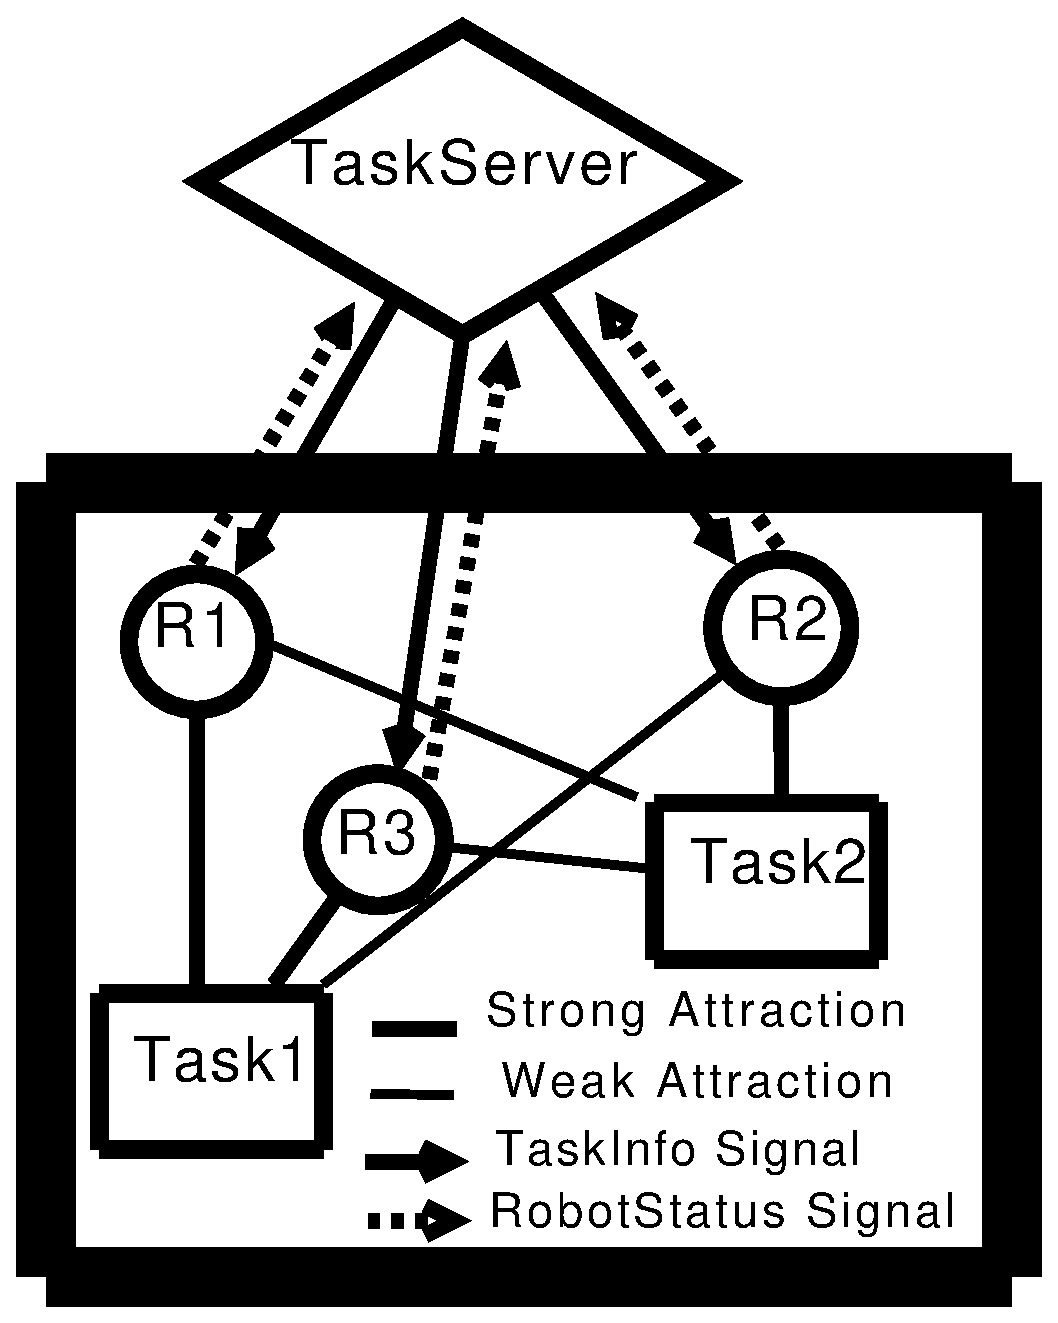
\includegraphics[height=4cm, angle=0]{./images/CentralizedComm.eps}
%\caption{\small A centralized communication scheme} % for implementing AFM}
%\label{fig:ccm} % Give a unique label
%\end{minipage}
\end{figure}
%%
AFM is presented graphically in Fig. \ref{fig:afm}.  The elements depicted are:
\begin{enumerate}
\item Source nodes (o) are tasks to be allocated to agents
\item Agent nodes (x) e.g., ants, humans, or robots
\item Black solid edges represent the attractive fields and correspond to an agent's perceived stimuli from each task.
\item Green edges represent the attractive field of the ever present no-task option, represented as a particular task (w).
\item The red lines are not edges, but represent how each agent is allocated to a single task at any point in time.
\end{enumerate}

The edges of the AFM network are weighted and the value of this weight describes the strength of the stimulus as perceived by the agent.  In a spatial representation of the model, the strength of the field depends on the physical distance of the agent to the source.  In information-based models, the distance can represent an agent's level of understanding of that task.  The strength of a field is increased through the sensitisation of the agent through experience with performing the task.  This elements is not depicted explicitly in Figure~\ref{fig:afm} but is represented in the weights of the edges.  In Figure~\ref{fig:afm}), the nodes have arbitrary positions.  Even though the distance is physical in this case, it need not be.  When the model is applied to other domains, the distance can represent the accessibility of information or the time the information takes to reach the agent. 
In summary, from the above diagram of the network, we can see that each of the agents is connected to each of the tasks. This means that even if an agent is currently involved in a task, the probability that it stops doing it in order to pursue a different task, or to random walk, is always non-zero.

AFM assumed a repeated task selection by individual agents.  The probability of an agent choosing to perform a task is proportional to the strength of the task's attractive field, as given by Equation~\ref{eqn:afm3}.
\begin{equation}
P_{j}^{i} = \frac{S_{j}^{i}}{\sum_{j=0}^{J} S_{j}^{i}} \hspace*{0.25cm}where,\hspace*{0.25cm}S^{i}_{0} = S^{i}_{RW}   
\label{eqn:afm3}
\end{equation}
Equation~\ref{eqn:afm3} states that the probability of an agent, $i$, selecting a task, $j$, is proportional to the stimulus, $ S^i_j$, perceived from that task, with the sum of all the task stimuli normalised to $1$.

The strength of an attractive field varies according to how sensitive the agent is to that task, $k_{j}^{i}$, the distance between the task and the agent, $d_{ij}$, and the {\em urgency}, $\phi _{j}$ of the task.  In order to give a clear edge to each field, its value is modulated by the hyperbolic tangent function, $tanh$.  Equation~\ref{eqn:afm1} formalises this part of AFM.
%% S
\begin{equation}
S_{j}^{i} = tanh\{\frac{k_{j}^{i}}{d_{ij}+\delta } \phi _{j}\}
\label{eqn:afm1}
\end{equation}
Eqation~\ref{eqn:afm1}, used small constant $\delta$, called {\em delta distance}, to avoid division by zero, in the case when a robot has reached to a task.

Equation~\ref{eqn:afm2} shows how AFM handles the the no-task, or random walk, option.  The strength of the stimuli of the random walk task depends on the strengths of the fields real tasks.  In particular, when the other tasks have a low overall level of sensitisation, i.e., relatively weak fields, the strength of the random walk field if relatively high.  On the other hand, when the agent is highly sensitised, the strength of the random walk field becomes relatively low.  We use $J$ to denote the number of real tasks.  AFM effectively considers random walking as an ever present additional task.  Thus the total number of tasks becomes $J+1$. %--P(Task)
\begin{equation}
S^{i}_{RW} = tanh \left \{ 1 -  \frac{ \sum_{j=1}^{J} S^{i}_{j}}{J + 1} \right \}
\label{eqn:afm2}
\end{equation}
%-- P(RW)

A task $j$ has an associated urgency $\phi_j$ indicating its relative importance over time.  If an agent attends a task $j$ in time step $t$, the value of $\phi_j$ will decrease by an amount $\delta_{\phi_{INC}}$ in the time-step $t+1$.  On the other hand, if a task has not been served by any of the agents in time-step $t$, $\phi_j$ will increase by a different amount, $\delta_{\phi_{DEC}}$ in time-step $t+1$.  This behaviour is formalised in Equations~\ref{eqn:delta-phi1} and~\ref{eqn:delta-phi2}.
\begin{equation}
 If\hspace*{0.15cm}the\hspace*{0.15cm} task\hspace*{0.15cm}is\hspace*{0.15cm}not\hspace*{0.15cm}being\hspace*{0.15cm} done:\hspace*{0.15cm} \phi_{j,t+1} \rightarrow \phi_{j,t} \hspace*{0.15cm} + \delta_{\phi_{INC}}
\label{eqn:delta-phi1}
\end{equation}
%%
\begin{equation}
 If\hspace*{0.15cm}the \hspace*{0.15cm}task\hspace*{0.15cm}is\hspace*{0.15cm}being\hspace*{0.15cm}done:\hspace*{0.15cm}  \phi_{j,t+1} \rightarrow \phi_{j,t} \hspace*{0.15cm} - n\hspace*{0.10cm}\delta_{\phi_{DEC}}
\label{eqn:delta-phi2}
\end{equation}
Equation~\ref{eqn:delta-phi1} refers to a case where no agent attends to task $j$ and Equation~\ref{eqn:delta-phi2} to the case where $n$ agens are concurrently performing task $j$.

In order to complete a task, an agent needs to be within a fixed distance of that task.  When an agent performs a task, it learns about it and this will increases the probability of that agent selecting that task in the future.  This is done by increasing its sensitization to the task by a fixed amount, $k_{INC}$. The variable affinity of an agent, $i$, to a task, $j$, is called its {\em sensitization} to that task and is denoted $k^{i}_{j}$.  If an agent, $i$, does not do a task $j$, $k^i_j$ is decreased by a different fixed amount, $k_{DEC}$.  This behaviour is formalised in Equations~\ref{eqn:k-inc} and~\ref{eqn:k-dec}.
\begin{equation}
 If\hspace*{0.15cm}task\hspace*{0.15cm}is\hspace*{0.15cm}done:\hspace*{0.15cm}  k^i_j \rightarrow   k^i_j \hspace*{0.15cm} + \hspace*{0.15cm} k_{INC}
\label{eqn:k-inc}
\end{equation}
\begin{equation}
 If\hspace*{0.15cm}task\hspace*{0.15cm}is\hspace*{0.15cm}not\hspace*{0.15cm}done:\hspace*{0.15cm}  k^i_j \rightarrow   k^i_j \hspace*{0.15cm} - \hspace*{0.15cm} k_{DEC}
\label{eqn:k-dec}
\end{equation}

%\subsection{A Robotic Interpretation of AFM}
%\label{afm:mrs-interpretation}
The interpretation of AFM in a multi-robot system follows the above mentioned generic interpretation.  The robots repeatedly select tasks and if the robot is outside a fixed task boundary, it navigates towards the task.  If the robot is within the task boundary it remains there until the end of the time step when a new (or the same) task is selected. The distance between a task and a robot is simply the physical distance and the sensitivities are recorded as specific values on each robot. The urgency values of the tasks are calculated based on the number of robots attending each task and the updated urgency values are communicated to the robots.

The sensing of the distance between the taks and robots as well as the communication of urgency values are non-trivial in a robotic systen.  Both the sensing and communication can be done either locally by the individual robots or centrally, through an overhead camera and a global communication network.
This article presents work on exploring the effects of different sensing and communication models on the performance of MRTA systems.
%%
\section{Related Work}
\label{sec:rw}
%%--------------------------------------------------------------------
%\subsection{AFM and Biological Self-Organization}
\label{afm:so}

Fig.  \ref{fig:afm-rules} labels the four distinct perspectives known as so-called ingredients or properties of self-organization:  A) positive feedback, B) negative feedback, C) presence of multiple interactions among individuals and their environment, and D) amplification of fluctuations  e.g., random walks, errors, random task-switching \cite{Camazine+2001}. However, it is not clear how those properties can come into existence. Fig.  \ref{fig:afm-rules} depicts  the four underlying mechanisms (label 1 to 4) that explain how self-organization can be realized in different social systems using our generic framework. These are explained in the following paragraphs.

Firstly, multiple interactions become meaningful when {\em continuous flow of information} occurs  by exchanging signals or cues among agents or their environment  that regulates their behaviours. This, in turn, contribute to the task-allocation  and task-switching in the social level.  In swarm intelligence literature, multiple interactions are often described as an essential ingredient of self-organization. However, interactions without definite purposes may not contribute to the self-organization.

Secondly, in swarm intelligence, positive feedback has been attributed as another mechanism of  self-organization. But it is not easy to understand what creates positive feedback in a social system. Possible answers might be the characteristic of the environment e.g. ants select shorter path since density of pheromones becomes higher and thus more ants becomes attracted in that path, by causing the gradual decrease of response-threshold of individuals. This increases the probability of selecting a task.  To make the answer more specific, we have explicitly attributed {\em sensitisation} or learning as a mechanism of positive feedback. There might exist other mechanisms too. But clearly sensitisation will be one of the reliable mechanisms for achieving positive feedback.

Thirdly, similar to positive feedback, we have proposed {\em forgetting} that contributes to provide negative feedback about a task or decreasing the probability to select it. Other negative feedback mechanisms can be implemented by assigning a saturation level to each task which is also present in our model, for details see \citet{Arcaute+2008}.

Finally, creating  artificial amplification of fluctuations or stochastic events is not a straight-forward issue. It throws  many open questions. Does a system designer intentionally impose irregularity in task-performance of agents?  Is random movement  enough for simulating randomness in a system?
Since emergencies do not always pop-up on request, we provide the rule of {\em concurrency} that enables agents to  maintain even a small amount of probability of selecting a low-priority, or less sensitized or distant task. This concurrency mechanism provides a high-degree of robustness in the system such that all tasks can be attended even if specialization of agents delays them in switching to some of the tasks.
%%
\begin{figure}[htp]
\centering
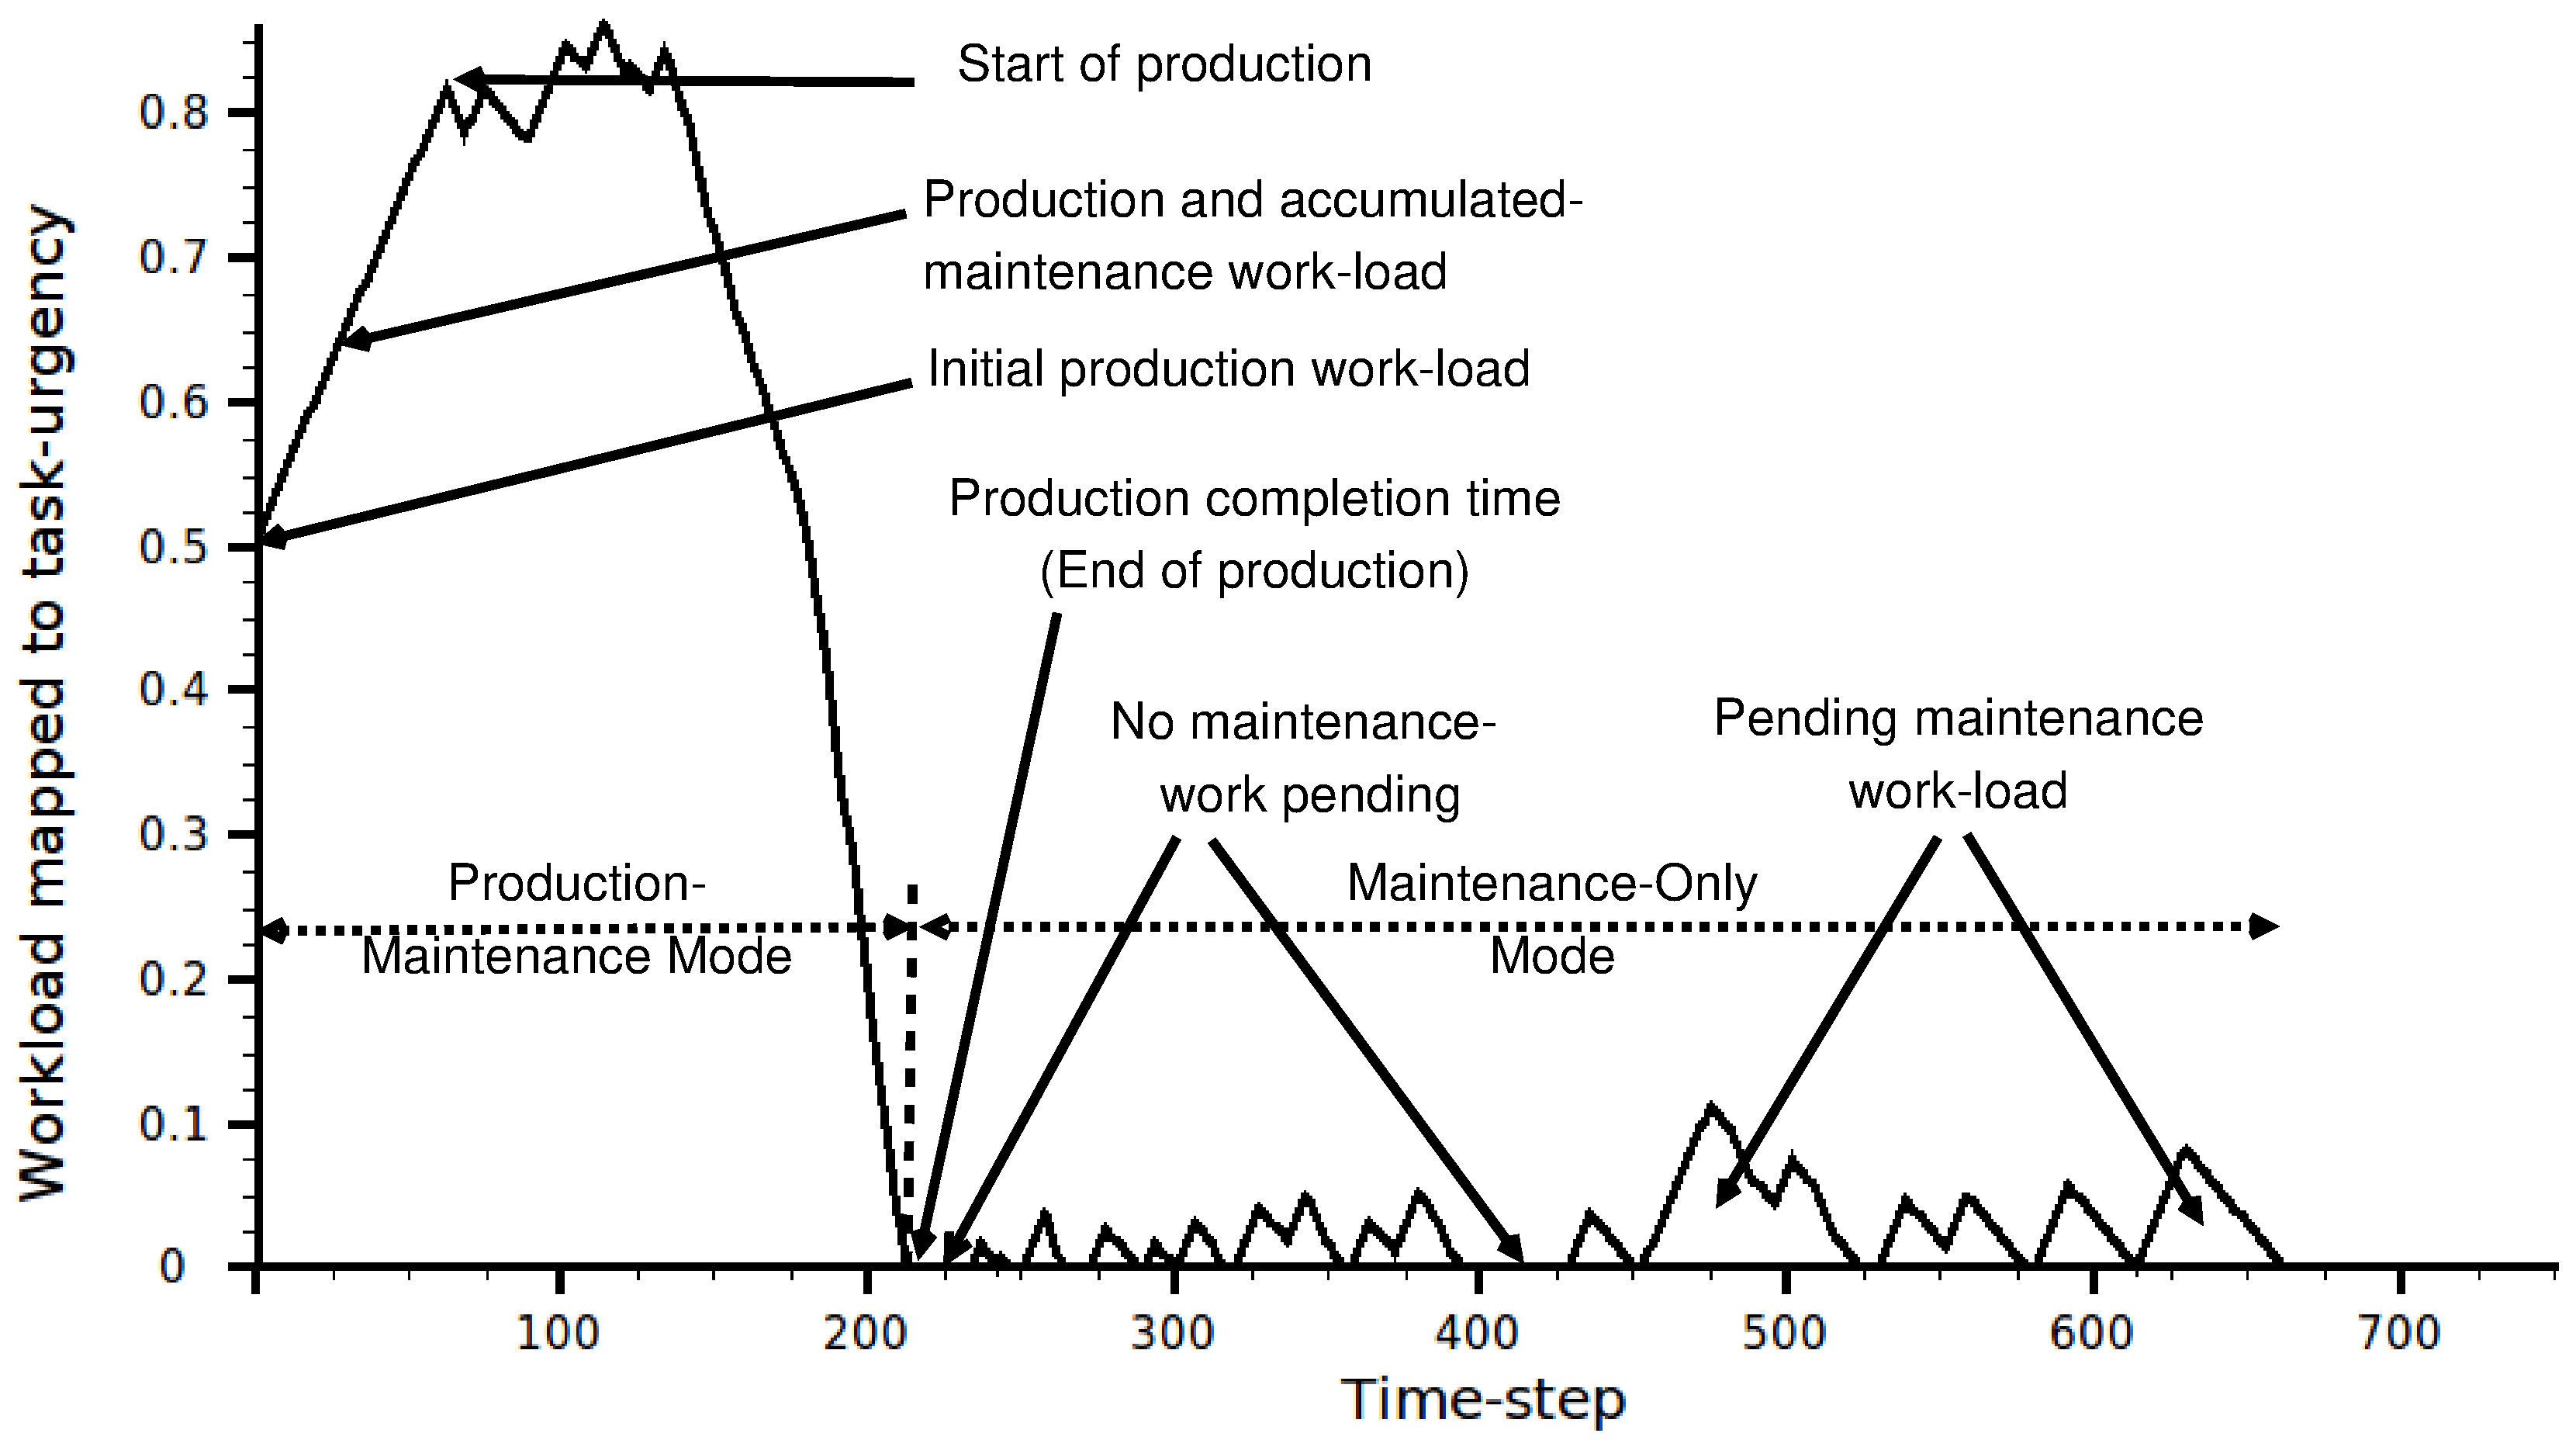
\includegraphics[width=12cm, angle=0]
{./images/VSP.eps}
%figure caption is below the figure
\caption{\small Virtual Shop-floor production and maintenance cycle}
\label{fig:vsp}  % Give a unique label
\end{figure}
%%
\subsection{A Manufacturing Shop-Floor Interpretation of AFM}
\label{sec:mrta}
We have designed a set of  manufacturing shop-floor scenario experiments for validating the effectiveness of our AFM in producing self-regulated MRTA. By extending our interpretation of AFM in multi-robot system, we can set-up manufacturing shop-floor  scenario. Here,, each task represents a manufacturing machine. These machines are capable of producing goods from raw materials, but they also require constant maintenance works for stable operations. Let $W_{j}$ be a finite number of material parts that can be loaded into a machine $j$ in the beginning of its production process and in each time-step, $\omega_{j}$ units of material parts can be processed  ($\omega_{j} \ll W_{j} $). So let $\Omega_{j}^{p}$ be the initial production workload of $j$ which is simply: $W_{j} / \omega_{j}$ unit. We assume that all machines are identical. In each time step, each machine always requires a minimum threshold number of robots, called hereafter as {\em minimum robots per machine ($\mu$)}, to meet its constant maintenance work-load, $\Omega_{j}^{m}$ unit. However, if $\mu$ or more robots are present in a machine for production purpose, we assume that, no extra robot is required to do its maintenance work separately. These robots, along with their production jobs, can do necessary maintenance works concurrently. For the sake of simplicity, in this paper we consider $\mu$ = 1.
Now let us fit the above production and maintenance work-loads and task performance of robots into a unit task-urgency scale. Let us divide our manufacturing operation into two subsequent stages: 1) {\em production and maintenance mode (PMM)}, and 2) {\em maintenance only mode (MOM)}. Initially a machine starts working in PMM and does production and maintenance works concurrently. When there is no production work left, it then enters into MOM. Fig. \ref{fig:vsp} illustrates this for a single machine.
Under both modes, let $\alpha_{j}$ be the amount of workload occurs in a unit time-step if no robot serves a task and it corresponds to a fixed task-urgency $\Delta \phi_{INC}$. On the other hand, let us assume that in each time-step, a robot, $i$, can decrease a constant workload $\beta_{i}$ by doing some maintenance work along with doing any available production work. This  corresponds to a negative task urgency: $- \Delta \phi_{DEC}$. 
So, at the beginning of production process, task-urgency, occurred in a machine due to its production work-loads, can be encoded by Eq. \ref{eqn:task-urgency-prod-init}.
\begin{equation}
%\small
\Phi_{j, INIT}^{PMM} = \Omega_{j}^{p} \times \Delta \phi_{INC} + \phi_{j}^{m0}
\label{eqn:task-urgency-prod-init}
\end{equation}
where $\phi_{j}^{m0}$ represents the task-urgency due to any initial maintenance work-load of $j$.
Now if no robot attends to serve a machine, each time-step a constant maintenance workload of $\alpha_{j}^{m}$ will be added to $j$ and that will increase its task-urgency by $\Delta \phi_{INC}$. So, if k time steps passes without any production work being done, task urgency at $k^{th}$ time-step will follow Eq. \ref{eqn:task-urgency-prod-case1}.
\begin{equation}
\Phi_{j, k}^{PMM} =\Phi_{j, INIT}^{PMM} + k \times \Delta \phi_{INC}
\label{eqn:task-urgency-prod-case1}
\end{equation}
However, if a robot attends to a machine and does some production works from it, there would be no extra maintenance work as we assumed that $\mu$ = 1. Rather, the task-urgency on this machine will decrease by $\Delta \phi_{DEC}$ amount. If $\nu_{k}$ robots work on a machine simultaneously at time-step $k$, this decrease will be: $\nu_{k} \times \Delta \phi_{DEC}$. So in such cases, task-urgency in $(k+1)^{th}$ time-step can be represented by:
\begin{equation}
\Phi_{j, k+1}^{PMM} = \Phi_{j, k}^{PMM} - \nu_{k} \times \Delta \phi_{DEC}
\label{eqn:task-urgency-prod-case2}
\end{equation}
At a particular machine $j$, once $\Phi_{j, k}^{PMM}$ reaches to zero, we can say that there is no more production work left and this time-step $k$ can give us the {\em production completion time} of $j$, $T_{j}^{PMM}$. Average production time-steps of a shop-floor with M machines can be calculated by the following simple equation.
\begin{equation}
T_{avg}^{PMM} = \frac{1}{M} \sum_{j=0}^{M} T_{j}^{PMM} 
\label{eqn:avg-pmm}
\end{equation}
$T_{avg}^{PMM}$ can be compared with the minimum number of time-steps necessary to finish production works, $T_{min}^{PMM}$. This can only happen in an ideal case where all robots work for production without any random walking or failure. We can get $T_{min}^{PMM}$ from the total amount of work load and maximum possible inputs from all robots. If there are M machines and N robots, each machine has $\Phi_{INIT}^{PMM}$ task-urgency, and each time-step robots can decrease N $\times$ $\Delta \phi_{DEC}$ task-urgencies, then the theoretical $T_{min}^{PMM}$ can be found from the following Eq. \ref{eqn:min-pmm}.
%
\begin{multicols}{2}
\small
\begin{equation}
T_{min}^{PMM} = \frac{M \times \Phi_{INIT}^{PMM}}{N \times \Delta \phi_{DEC}} 
\label{eqn:min-pmm}
\end{equation}
\vspace*{0.2cm}
\begin{equation}
\zeta_{avg}^{PMM} = \frac{T_{avg}^{PMM} - T_{min}^{PMM}}{T_{min}^{PMM}} 
\label{eqn:appd}
\end{equation}
\end{multicols}
Thus we can define $\zeta_{avg}^{PMM}$, {\em average production completion delay} (APCD) by following Eq. \ref{eqn:appd}:
%%
When a machine enters into MOM, only $\mu$ robots are required to do its maintenance works in each time step. So, in such cases, if no robot serves a machine, the growth of task-urgency will follow Eq. \ref{eqn:task-urgency-prod-case1}. However, if $\nu_{k}$ robots are serving this machine at a particular time-step $k^{th}$ , task-urgency at $(k+1)^{th}$ time-step can be represented by:
\begin{equation}
\Phi_{j, k+1}^{MOM} = \Phi_{j, k}^{MOM}- (\nu_{k} - \mu) \times \Delta \phi_{DEC}
\label{eqn:task-urgency-maint-case}
\end{equation}
By considering $\mu = 1$ Eq. \ref{eqn:task-urgency-maint-case} will reduces to Eq. \ref{eqn:task-urgency-prod-case2}. Here, $\Phi_{j, k+1}^{MOM}$ will correspond to the {\em pending maintenance work-load (PMW)} of a particular machine at a given time. This happens due to the random task switching of robots with a no-task option (random-walking). Interestingly PMW will indicate the robustness of this system since higher PMW value will indicate the delay in attending maintenance works by robots. We can find the average PMW (APMW) per time-step per machine, $\chi_{j}^{MOM}$ (Eq. \ref{eqn:sigle-pmw}) and average PMW per machine per time-step, $\chi_{avg}^{MOM}$ (Eq. \ref{eqn:avg-pmw}).
\begin{multicols}{2}
\small
\begin{equation}
\chi_{j}^{MOM}= \frac{1}{K} \sum_{k=1}^{K} \Phi_{j, k}^{MOM}
\label{eqn:sigle-pmw}
\end{equation}
\vspace*{0.2cm}
\begin{equation}
\chi_{avg}^{MOM}= \frac{1}{M} \sum_{j=1}^{M} {\chi_{j}^{MOM}}
\label{eqn:avg-pmw}
\end{equation}
\end{multicols}
%%=========================================================
\section{Centralized Communication Scheme}
\label{sec:comm}
\begin{figure}
\centering
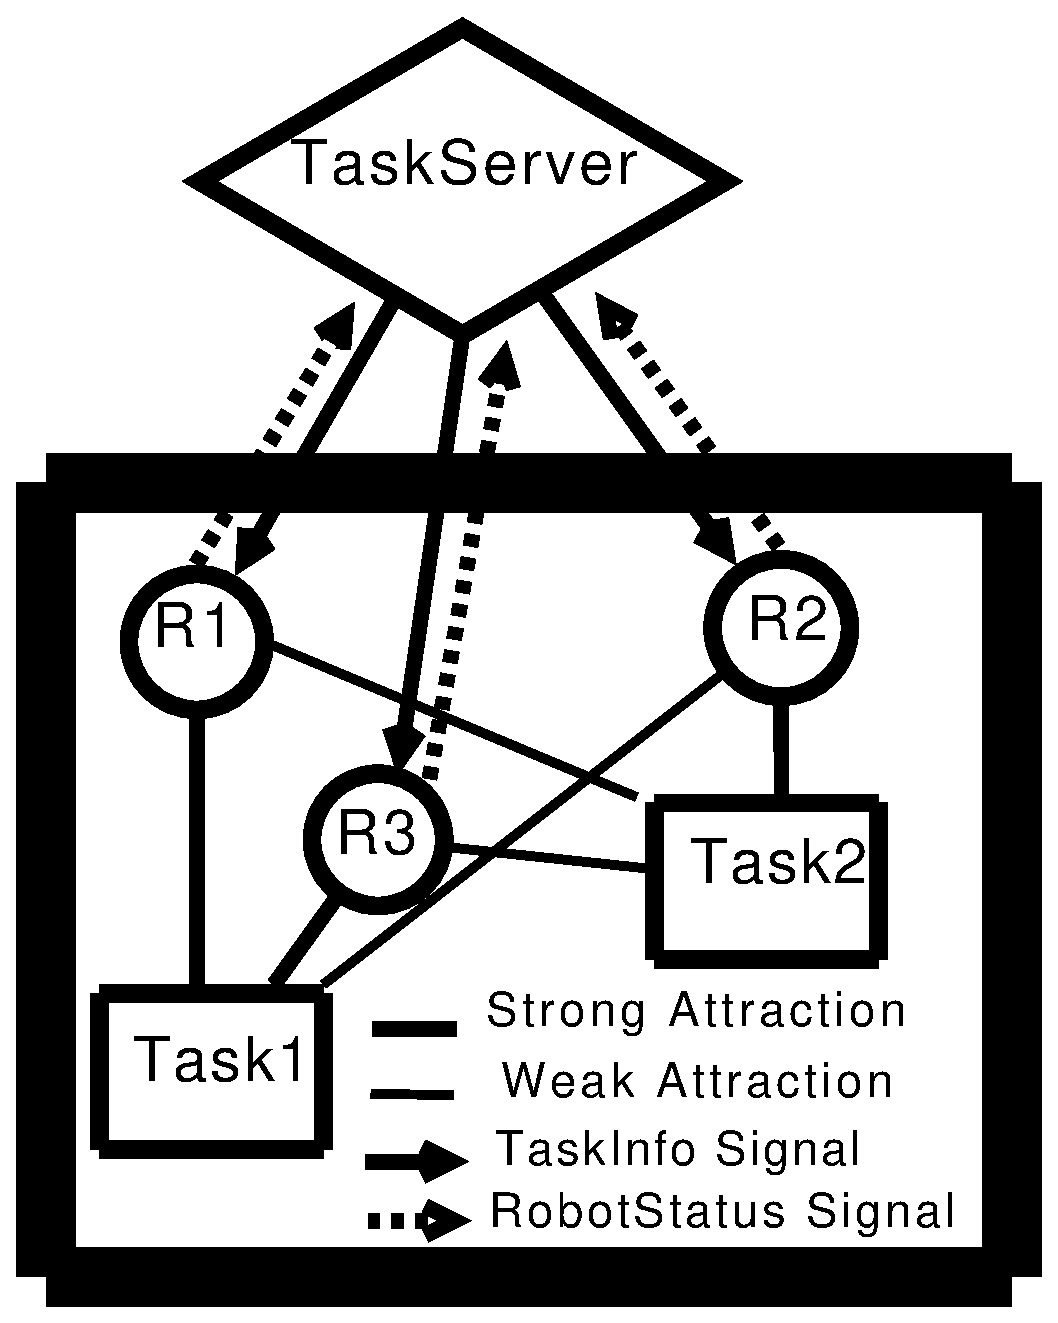
\includegraphics[height=5cm, angle=0]{./images/CentralizedComm.eps}
\caption{\small A centralized communication scheme} % for implementing AFM}
\label{fig:ccm} % Give a unique label
\end{figure}
%%
AFM relies upon a system-wide continuous flow of information which can be realized using any suitable communication model. A simple centralized communication scheme is outlined in Fig. \ref{fig:ccm}. In this model we have used bi-directional signal-based exchange of communication messages between a centralized \textit{task perception server} (TPS) and a \textit{robot-controller client} (RCC). The main role of TPS is to send up-to-date task-information to RCCs. This  task-information mainly contains the location and urgency of all tasks  which is used by the RCCs for running their task-allocation algorithm. The urgency value of each task is dynamically updated  by TPS after receiving the  status signals from the working robots of that particular task. Fig. \ref{fig:ccm} shows how three robots are attracted to two different tasks and their communications with TPS.

We can characterize our communication model in terms of three fundamental issues of communication: 
i) message content, ii) communication frequency and iii) target message recipients \citep{Gerkey+2001}.
%%
AFM suggests the communication of task-urgencies  among robots. This communication helps the robots to gain information that can be  treated as ``global sensing''. However in this model  robots do not communicate among themselves. Since in order to run the task-allocation algorithm robot-controllers need the distance information we also include the task position information in  the message. Our centralized communication model is open to include any further information, such as time-stamp, in the message payload. In this model the frequency of signal emission depends on several issues, e.g. the rate at which the environment is changing, the bandwidth of communication medium. In case of time-extended tasks, robots can receive information less frequently and the  bandwidth usage can be kept  minimum. However under a fast changing environment relatively more bandwidth will be required.  Finally the centralized communication model spread the attractive fields of all tasks globally by broadcasting information to all robots.  
%%%%%%%%%%%%%%%%%%%%%%%%%%%%%%%%%%%%%%%%%%%%%%%%%%%%%%%%%%%%%%%%%%%%%%%%%%%%
\section{Experiments}
\label{sec:expt}
In this section, we have described the design of parameters and observables of our experiments within the context of our virtual manufacturing shop-floor scenario. 
These experiments are designed to validate AFM by testing the presence of division of labour, such task specialization, dynamic task-switching or plasticity etc. 
\subsection{Observables}
\textbf{Plasticity:} %As we have discussed in Sec. \ref{bg:def:dol},  
Self-regulated MRTA is often characterised by the plasticity and task-specialization, in both macroscopic and microscopic levels. Within our manufacturing shop-floor context, plasticity refers to the collective ability of the robots to switch from doing no-task option (random-walking) to doing a task (or vice-versa) depending on the work-load present in the system. Here we expect to see that most of the robots would be able to engage in tasks when there would be high workloads (or task-urgencies) during PMM. Similarity, when there would be low workload in case of MOM, only a few robots would do the task, rest of them would either be idle (not doing any task) or perform a random-walk.  The changes of task-urgencies and the ratio of robots engaged in tasks can be good metrics to observe plasticity in MRTA.

\textbf{Task-specialization:} Self-regulated MRTA is generally accompanied with task-specializations of agents. That means that few robots will be more active than others. From the interpretation of AFM, we can see that after doing a task a few times, a robot will soon be sensitized to it. Therefore, from the raw log of task-sensitization of robots, we can be able to find the pattern of task-sensitization of robots per task basis.

\textbf{Quality of task-performance:} As discussed in Sec. \ref{afm:vms} we can measure the quality of MRTA from the APCD. It first calculates the ideal minimum production time and then finds the delay in production process from the actual production completion data. Thus this will indicate how much more time is  spent in the production process due to the self-regulation of robots in this distributed task-allocation scheme.  In order to calculate APCD, we can find the production completion time for each task from the raw log of task-urgency and make an average from them.

\textbf{Robustness:} In order to see if our system can respond to the gradually increasing workloads,  we can measure APMW within the context of our manufacturing shop-floor scenario. This can show the robustness of our system. When a task is not being served by any robot for some time we can see that its urgency will rise and robots will respond to this dynamic demand. For measuring APMW we need only the task-urgency data.

\textbf{Flexibility:} From the design of AFM, we know that robots that are not doing a task will be de-sensitized to it or forget that task. So at an overall low work-load (or task urgency), less robots will do the tasks and hence less robots will have the opportunity to learn tasks. From the shop-floor work-load data, we can confirm the presence of flexibility in MRTA.

\textbf{Energy-efficiency:} In order to characterize the energy-efficiency in MRTA we can log the pose data of each robot that can give us the total translations occurred by all robots in our experiments. This can give us a rough indication of energy-usage by our robots. 

\textbf{Information flow:} Since AFM requires a system-wide continuous flow of information, we can measure the communication load to bench-mark our implementation of communication system. This bench-mark data can be used to compare among various communication strategies. Here we can measure  how much task-related information, i.e. task-urgency, location etc. are sent to the robots at each time step. This  amount of information or communication load can be constant or variable depending on the design of the communication system.

\textbf{Scalability:} In order to see the effects of scaling on MRTA, we have designed two group of experiments. Series A corresponds to a small group where we have used 8 robots, 2 tasks under an arena of 2 $m^2$. We have doubled these numbers in Series B, C and D, i.e. 16 robots, 4 tasks under an arena of 4 $m^2$. This proportional design can give us a valuable insight about the effects of scaling on self-regulated MRTA. 

Thus, in order to observe the above properties of self-regulated MRTA , we have designed our experiments to record the following  observables in each time-step.
\begin{enumerate}
\item Task-urgency of each task ($\phi$).
\item Number of robots engaged in each task.
\item Task-sensitizations ($k$) of robots.
\item Pose data of robots.
\item Communication of task-information message among TPS and RCCs.  
\end{enumerate}
%%
\begin{table}
\caption{Experimental parameters of Series A \& B experiments}
\label{table:params}
\begin{center}
\begin{tabular}{|p{2in}|c|}
\hline Parameter & Series A $\mid$ Series B\\
\hline Total number of robots ($N$) & \hspace*{0.1cm} 8 $\mid$ 16\\
\hline Total number of tasks ($M$) & 2 $\mid$ 4\\
\hline Experiment area ($A$) & 2 $m^2$ $\mid$  4 $m^2$\\
\hline Initial production work load/machine ($\Omega_{j}^{p}$) & 100 unit \\
\hline Task urgency increase rate ($\Delta\phi_{INC}$) & 0.005\\
\hline Task urgency decrease rate ($\Delta\phi_{DEC}$) & 0.0025\\
\hline Initial sensitization ($K_{INIT}$) & 0.1\\
\hline Sensitization increase rate ($\Delta k_{INC}$) & 0.03\\
\hline Sensitization decrease rate ($\Delta k_{DEC}$) & 0.01\\
\hline
\end{tabular}
\end{center}
\end{table}
%%
%------------------------------------------------------------
\subsection{Parameters}
Table \ref{table:params} lists a set of essential parameters of our GSNC startegy based experiments (Series A and B). We intend to have a set-up that is relatively complex, i.e., with a high number of robots and tasks in a large area. The diameter of the marker of our e-puck robot is 0.08m (Fig \ref{fig:e-puck}). So, if we put 4 robots in an area of one square meter, this will give us a robot-occupied-space to free-space ratio of about 1:49 per square meter. This ratio is reasonable in order to allow the robots to move at a speed of 5 cm/sec without causing much interference to each other. 

The initial values of task urgencies correspond to 100 units of production work-load without any maintenance work-load as outlined in Eq. \ref{eqn:task-urgency-prod-init}. We choose a limit of 0 and 1, where 0 means no urgency and 1 means maximum urgency. Same rule applies to sensitisation, where 0 means no sensitisation and 1 means maximum sensitisation. This also implies that if sensitization is 0, task has been forgotten completely. On the other hand, if sensitization is 1, the task has been learnt completely. We choose a initial sensitization value of 0.1 for all tasks. The following relationships are maintained for selecting task-urgency and sensitization parameters.
\begin{equation}
\Delta\phi_{INC} = \frac{\Delta\phi_{DEC} \times N}{2 \times M}
\label{eqn:task-urgency}
\end{equation}
%
\begin{equation}
\Delta k_{DEC} = \frac{\Delta k_{INC}} {M - 1} 
\label{eqn:sensitization}
\end{equation}
%
Eq. \ref{eqn:task-urgency} establishes the fact that task urgency will increase at a higher rate than that of its decrease. As we do not like to keep a task left unattended for a long time we choose a higher rate of increase of task urgency. This difference is set on the basis of our assumption that at least half of the expected number of robots (ratio of number of robots to tasks) would be available to work on a task. So they would produce similar types of increase and decrease behaviours in task urgencies.

Eq. \ref{eqn:sensitization} suggests that the learning will happen much faster than the forgetting. The difference in these two rates is based on the fact that faster leaning gives a robot more chances to select a task in next time-step and thus it becomes more specialized on it.
%%%%%%%%%%%%%%%%%%%%%%%%%%%%%%%%%%%%%%%%%%%%%%%%%%%% 
\subsection{Implementation}
\label{sec:impl}
\begin{figure}
\centering
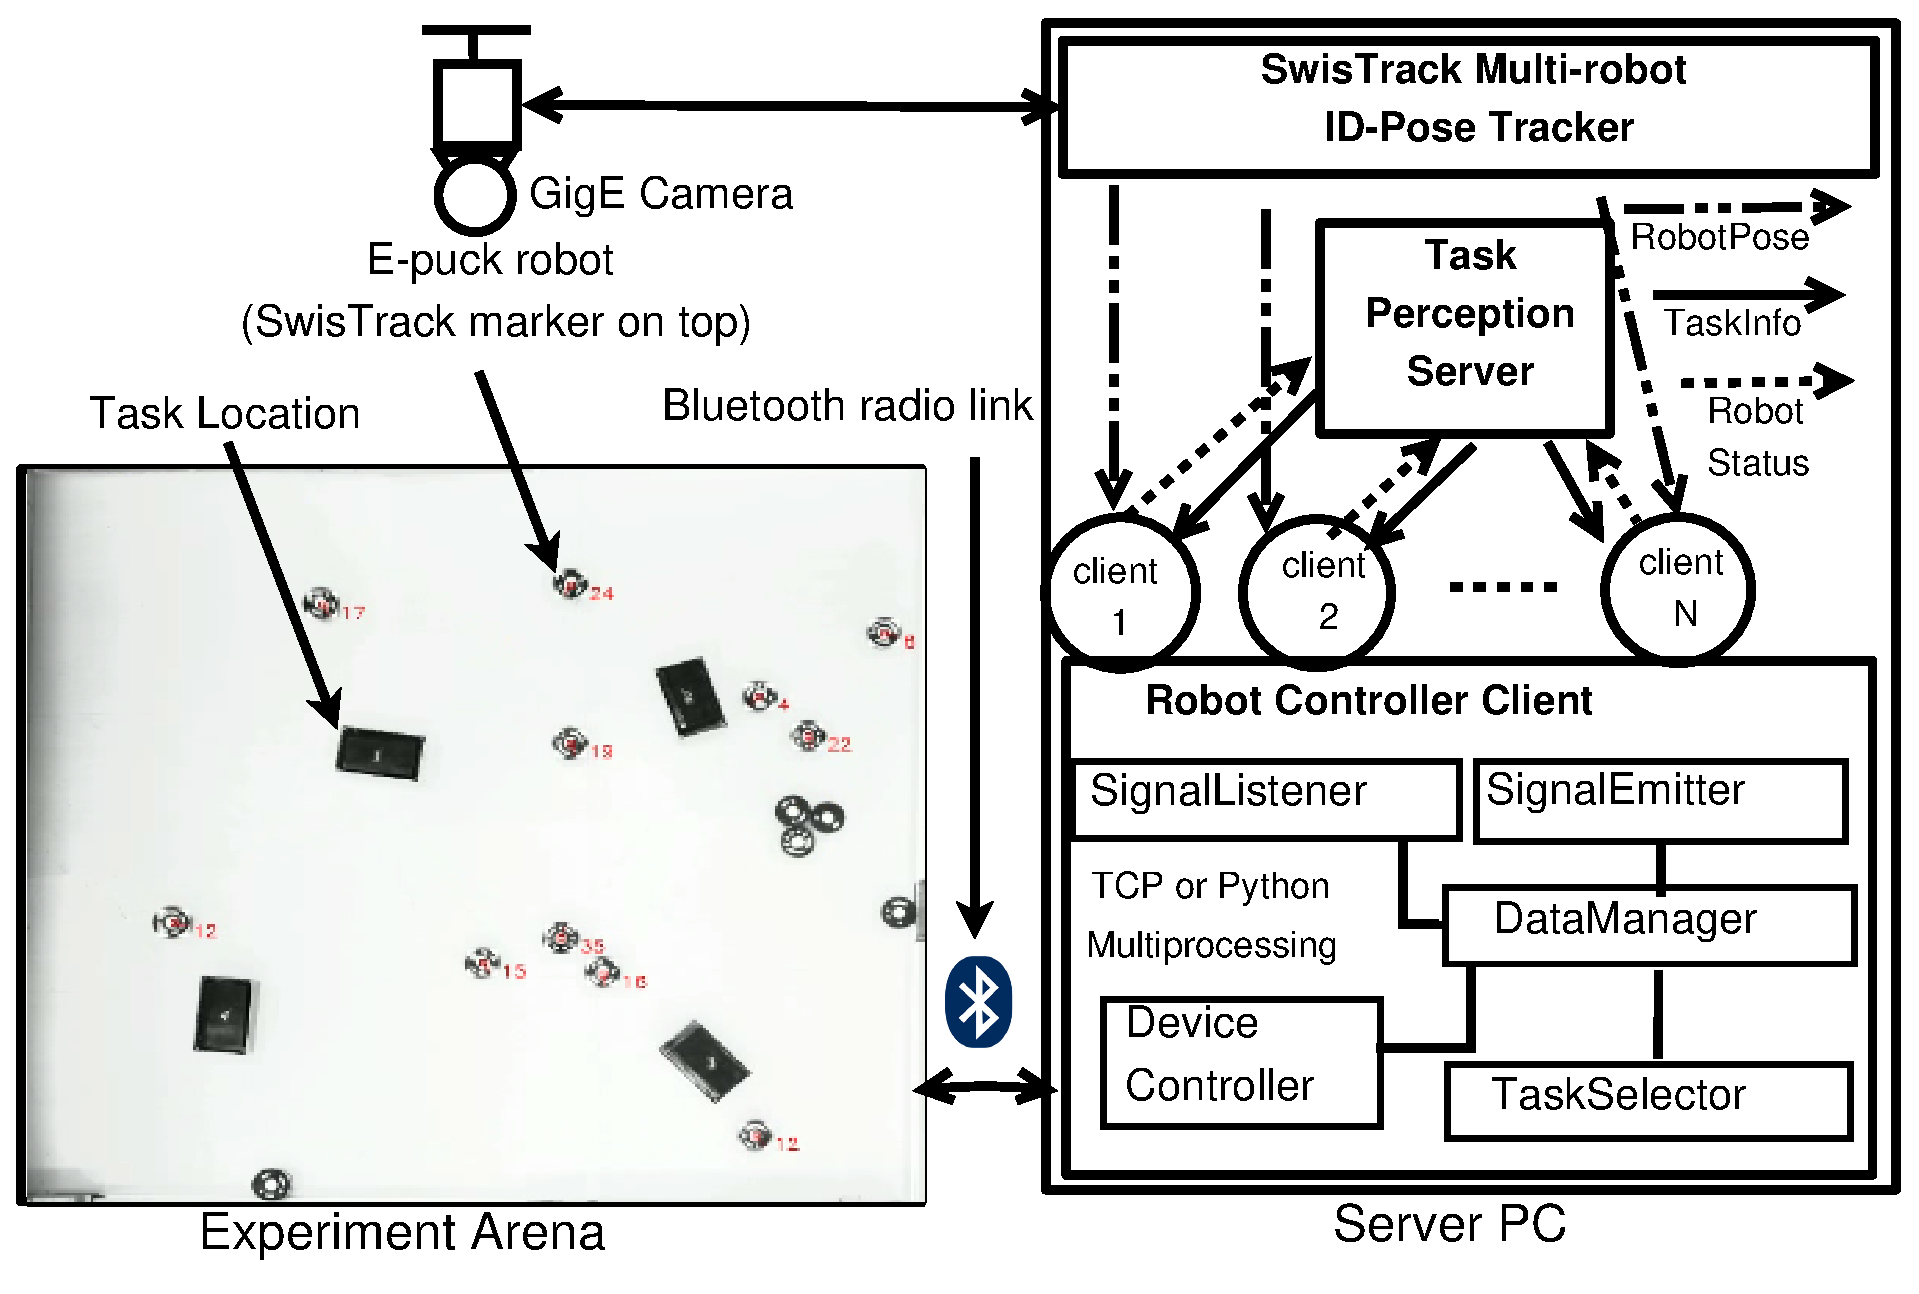
\includegraphics[height=5cm, angle=0]
{./images/RIL-Expt-Setup1.eps}
%figure caption is below the figure
\caption{\small Hardware and software setup}
\label{fig:setup} % Give a unique label
\end{figure}
We have developed a system a multi-robot tracking system can track at least 40 E-puck robots \footnote{www.e-puck.org} and these robots can operate together according to the generic rules of the AFM.
As shown in Fig. \ref{fig:setup}, our software system consists of a multi-robot tracking system, a centralized task server and robot controller clients. Here at first we have presented the design of our communication system. Then we have discussed about our specific implementation. 
%%%
\subsection{Design of our communication system}
In order to establish a system-wide continuous flow of information, we need to implement a suitable communication system for our robots. Here we have presented a centralized communication system for our manufacturing shop-floor scenario.
%% 
As shown in Fig. \ref{fig:ccm}, in this model there exists a centralized \textit{
TaskServer} that is responsible for disseminating task information to robots. The contents of task information can be physical locations of tasks, their urgencies and so on. TaskServer delivers this information by emitting \textit{TaskInfo} signals periodically. The method of signal emission depends on a particular communication technology. For example, in a wireless network it can be a message broadcast.
Task-Server has another interface for catching feedback signals from robots. The \textit{RobotStatus} signal can be used to inform TaskServer about a robot's current task id, its device status and so on. TaskServer uses this information to update relevant part of task information such as, task-urgency. This up-to-date information is sent in next TaskInfo signal.\\
In Fig. \ref{fig:ccm} an initial configuration of this model has been presented. Upon receiving an initial TaskInfo signal robot $R_1$ has shown strong attraction towards $Task1$ and robot $R_3$ has shown strong attraction toward $Task2$. This can be inferred from Eq. \ref{eqn1} that says if the initial task urgencies and sensitizations for all tasks are same, a robot will strongly be attracted towards a task that is relatively closer to it.
\subsection{Our current implementation}
The major components of our implementation are a multi-robot tracking system, robot controller clients and a centralized task-server. In order to track all robots real-time we have used SwisTrack \citep{Lochmatter+2008}, a state of the art open-source, multi-agent tracking system, with a16-megapixel overhead GigE camera. This set-up gives us the position, heading and id of each of the robots at a frequency of 1. The interaction of the hardware and software of our system is illustrated in Fig. \ref{fig:setup}. \\
For inter-process communication (IPC), we have used D-Bus technology \footnote{http://dbus.freedesktop.org/doc/dbus-specification.html}. We have developed an IPC component for SwisTrack (hereafter called as \textit{SwisTrack D-Bus Server}) that can broadcast id and pose of all robots in real-time over our server's D-Bus interface.\\
Apart from SwisTrack, we have implemented two major software modules: {\em TaskServer} and {\em Robot Controller Client (RCC)}. They are developed in Python with its state of the art \textit{Multiprocessing} \footnote{http://docs.python.org/library/multiprocessing.html} module. This python module simplifies our need to manage data sharing and synchronization among different sub-processes. As shown in Fig. \ref{fig:setup}, RCC consists of four sub-processes. {\em SignalListener} and {\em SignalEmitter}, interface with SwisTrack D-Bus Server and TaskServer respectively. {\em TaskSelector} implements AFM guidelines for task selection . {\em DeviceController} moves a robot to a target task. Bluetooth radio link is used as a communication medium between a RCC and a corresponding E-puck robot. 

%================================================================= 
\section{Results and Discussions}
\label{sec:res}
%%
In this section we have presented our experimental results. We ran those experiments for about 40 minutes and averaged them over five iterations.
Fig. \ref{fig:raw-urgencies} shows the dynamic changes in task urgencies.  In order to describe our system's dynamic behaviour holistically we analyse the changes in task urgencies over time. Let $ \phi_{j, q}$ be the urgency of a task $j$ at $q^{th}$ step and $\phi_{j, q+1}$ be the task urgency of $(q+1)^{th}$ step. We can calculate the sum of changes in urgencies of all tasks at $(q+1)^{th}$ step:
\begin{equation} 
\small
\Delta \Phi_{j, q+1} = \sum_{j=1}^{M} (\phi_{j, q+1} - \phi_{j, q})
\label{eqn:Delta-Phi}
\end{equation}
From Fig. \ref{fig:urgency-stat} we can see that initially the sum of changes of task urgencies are towards negative direction. This implies that tasks are being served by a high number of robots. Fig. \ref{fig:worker-stat} shows that in production stage, when  work-load is high, many robots are active in tasks and this ratio varies according to task urgency changes.\\ 
Fig. \ref{fig:single-robot-sensitizations} gives us the task specialization of five robots on Task3 in a particular run of our experiment. This shows us how our robots can specialize and de-specialize on tasks over time. The de-specialization or forgetting of tasks is calculated similar to Eq. \ref{eqn:Delta-Phi}. we have calculated the absolute sum of changes in sensitizations by all robots in the following equation.
% 
\begin{equation}
\small 
\Delta K_{j, q+1} = \sum_{j=1}^{M} \left | (k_{j, q+1} - k_{j, q}) \right |
\label{eqn:Delta-K}
\end{equation}
This values of $\Delta K$ are plotted in Fig. \ref{fig:sensitization-stat}. It shows that the overall rate of learning decreases and forgetting increases over time. It is a consequence of the gradually increased task specialization of robots and reduced task-urgencies over time.
%%
%%% Communication load %%%
Fig. \ref{fig:signal-frequency-stat} presents the frequency of signalling task information by TaskServer. Since the duration of each time step is 50s long and TaskServer emits signal in every 2.5s, there should be an average of 20 signals in each time-step.\\
Within VMS scenario, we have got average production completion time 165 time-steps (825s) where sample size is (5 x 4) =  20 tasks, SD = 72 time-steps (360s). According to Eq. \ref{eqn:min-pmm}, our theoretical minimum  production completion time is 50 time-steps (250s) assuming the non-stop task performance of all 16 robots with an initial task urgency of 0.5 for all 4 tasks and  task urgency decrease rate $\Delta \Phi_{DEC	}$ = 0.0025 per robot per time-step. Hence, Eq. \ref{eqn:appd} gives us APCD, $\zeta$ = 2.3 which means that our system has taken 2.3 times more time (575s) than the minimum estimated time.\\
Besides,  from the average 315 time-steps (1575s) maintenance activity of our robots per experiment run, we have got  APMW, $\chi$ = 0.012756  which corresponds to the pending work of 3 time-steps (15s) with sample-size = 20 tasks, SD = 13 time-steps (65s), $\Delta \Phi_{INC}$ = 0.005 per task per time-step. This tells us the robust task performance of our robots which can return to an abandoned task within a minute or so.
%%
\begin{figure}
\begin{minipage}[t]{0.48\linewidth}
\centering
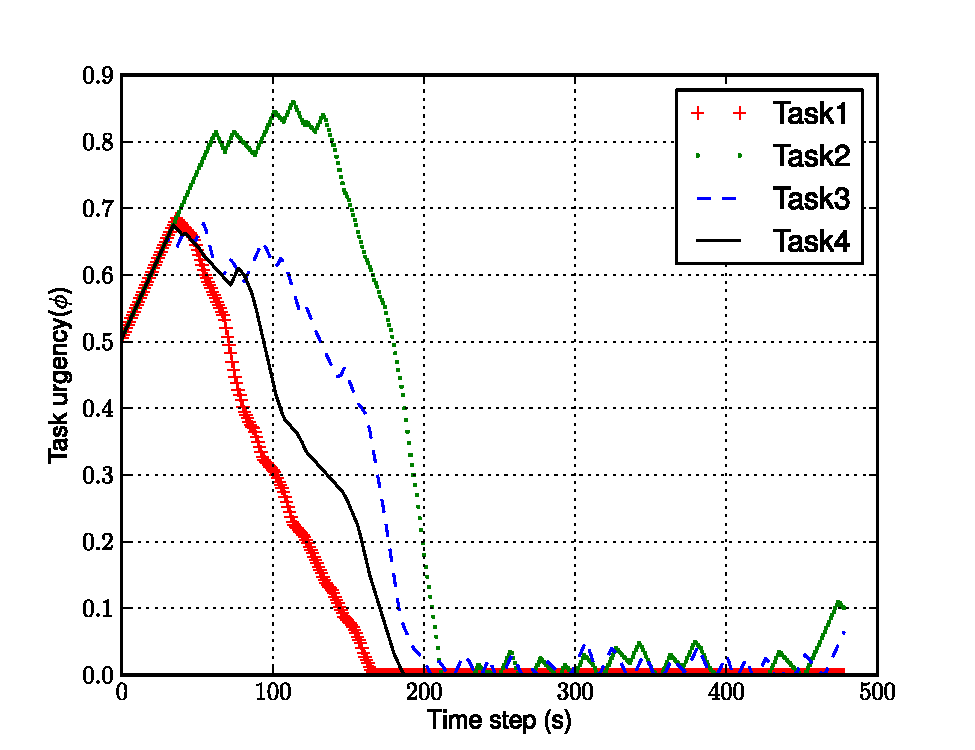
\includegraphics[height=4.5cm, angle=0]
{images/PlotUrgencyLog-2010May10-115549.eps}
%figure caption is below the figure
\caption{\small Task urgencies observed at TaskServer}
\label{fig:raw-urgencies} % Give a unique label
\end{minipage}
\hspace{0.5cm}
\begin{minipage}[t]{0.48\linewidth}
\centering
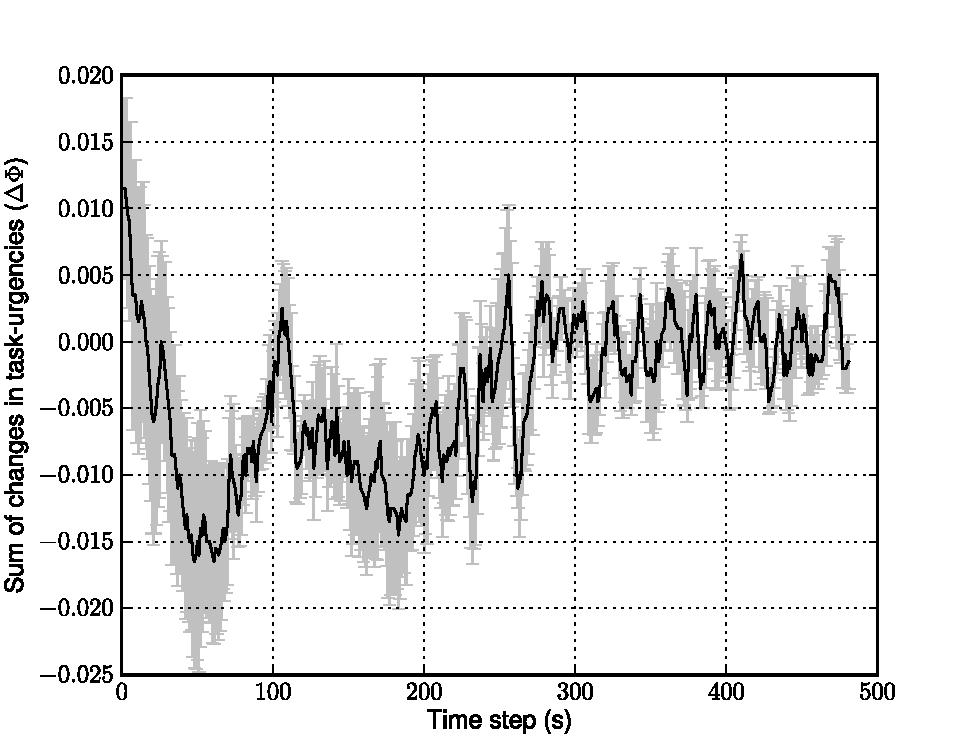
\includegraphics[height=4.5cm, angle=0]{images/TaskUrgencyStat.eps}
\caption{\small Shop-floor workload change history} % measured in terms of task urgencies
\label{fig:urgency-stat} % Give a unique label
\end{minipage}
\end{figure}
%%
%%% Sensitization and Translation %%%
\begin{figure}
\begin{minipage}[t]{0.48\linewidth}
\centering
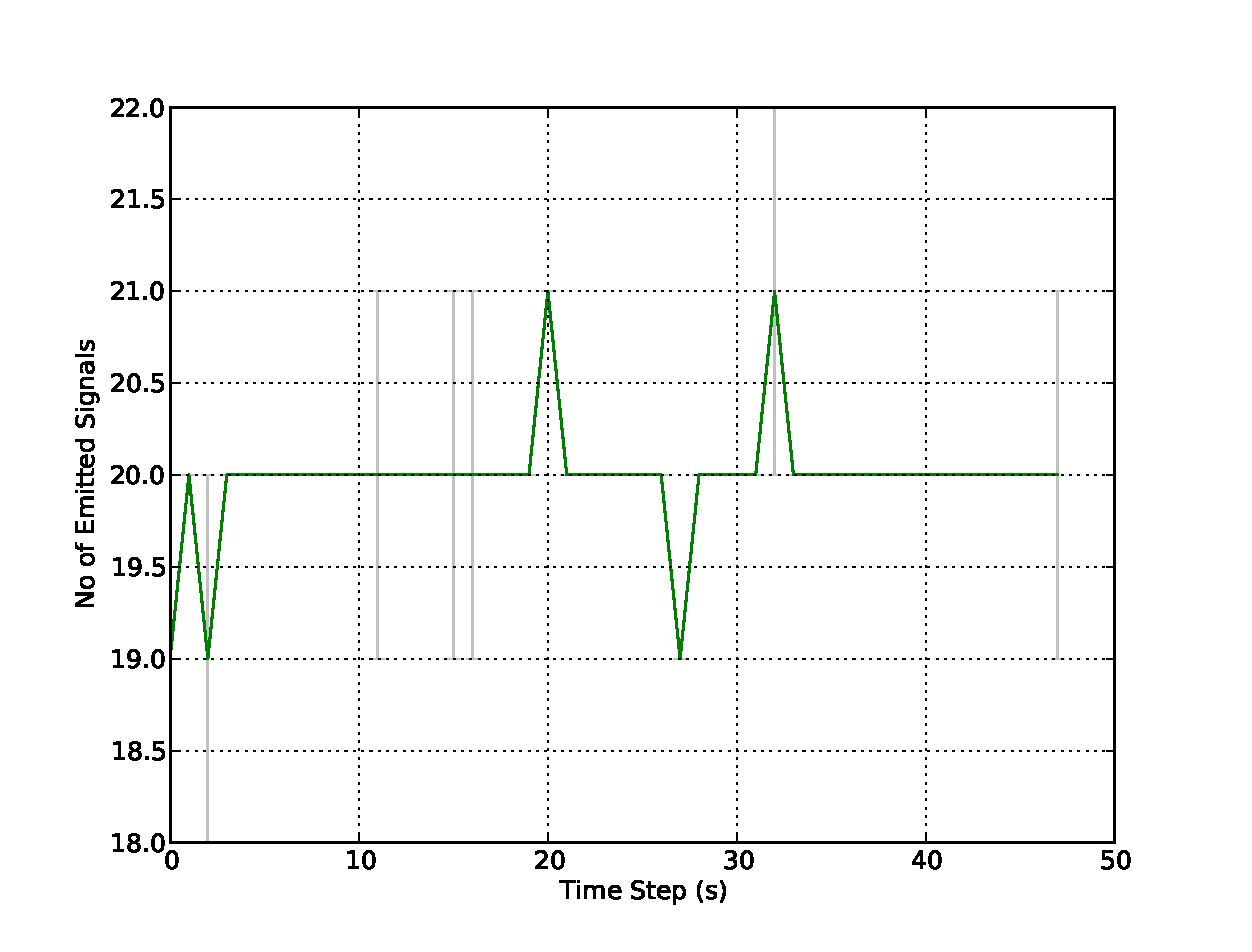
\includegraphics[height=4.5cm, angle=0]
{images/Global-SignalingFreqStat.eps}
%figure caption is below the figure
\caption{\small Task server's frequency of task information signalling}
\label{fig:signal-frequency-stat}
%
\end{minipage}
\hspace{0.5cm}
\begin{minipage}[t]{0.48\linewidth}
\centering
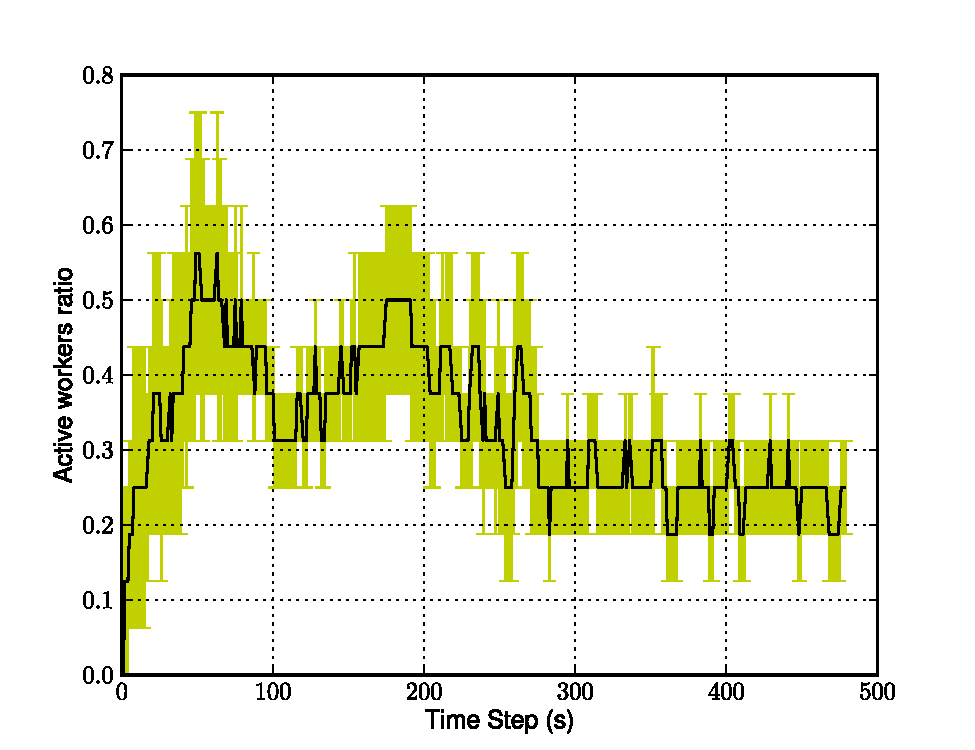
\includegraphics[height=4.5cm, angle=0]{images/WorkerRatio.eps}
\caption{\small Self-organized allocation of workers }
\label{fig:worker-stat} % Give a unique label
\end{minipage}
\end{figure}
%%
\begin{figure}
\begin{minipage}[t]{0.48\linewidth}
\centering
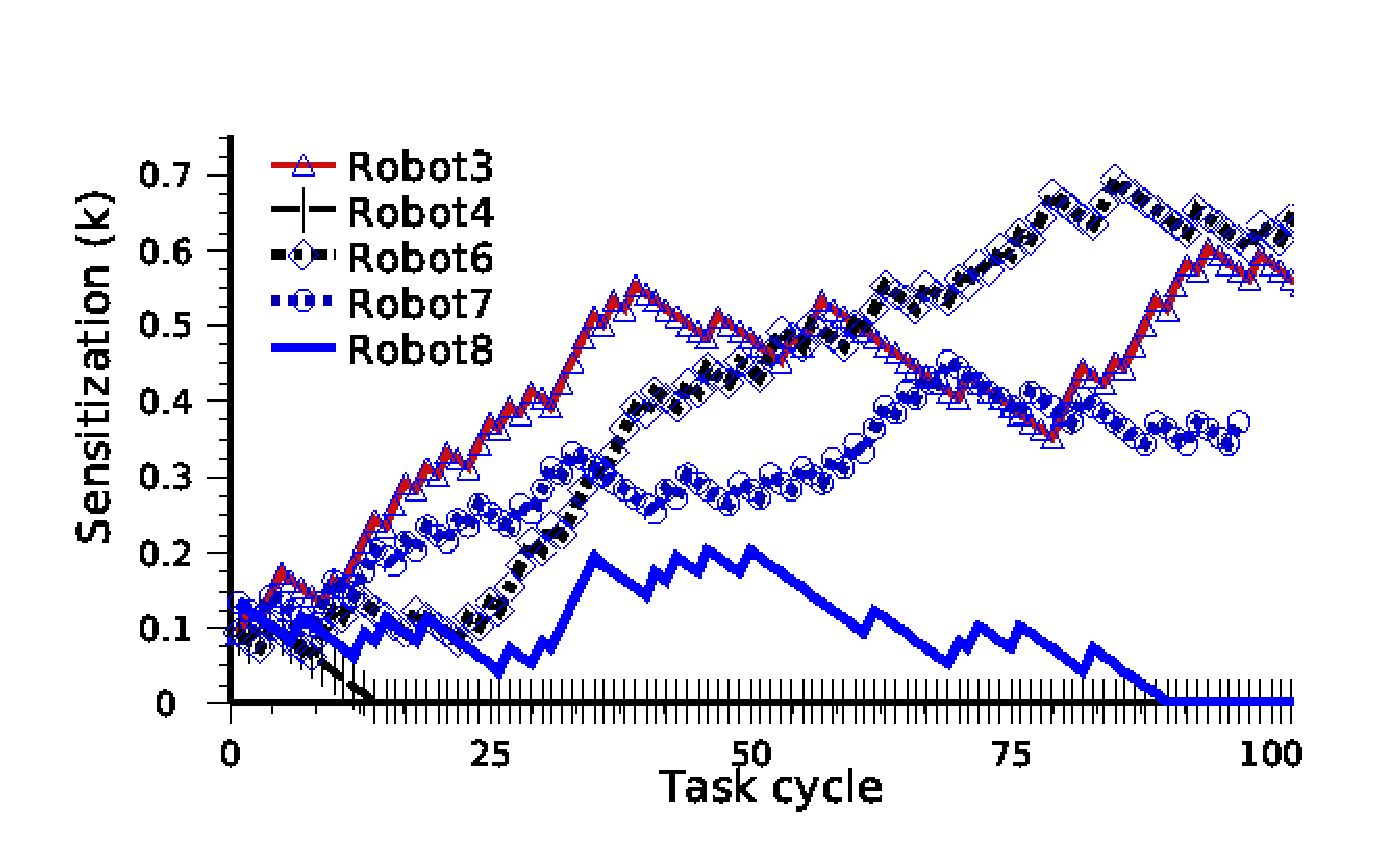
\includegraphics[height=4cm, angle=0]{images/TaskSpecialization-task3-10may-1.eps}
\caption{\small Task specialization on Task3}
\label{fig:single-robot-sensitizations} % Give a unique label
\end{minipage} 
%%%
\hspace{0.5cm}
\begin{minipage}[t]{0.48\linewidth}
\centering
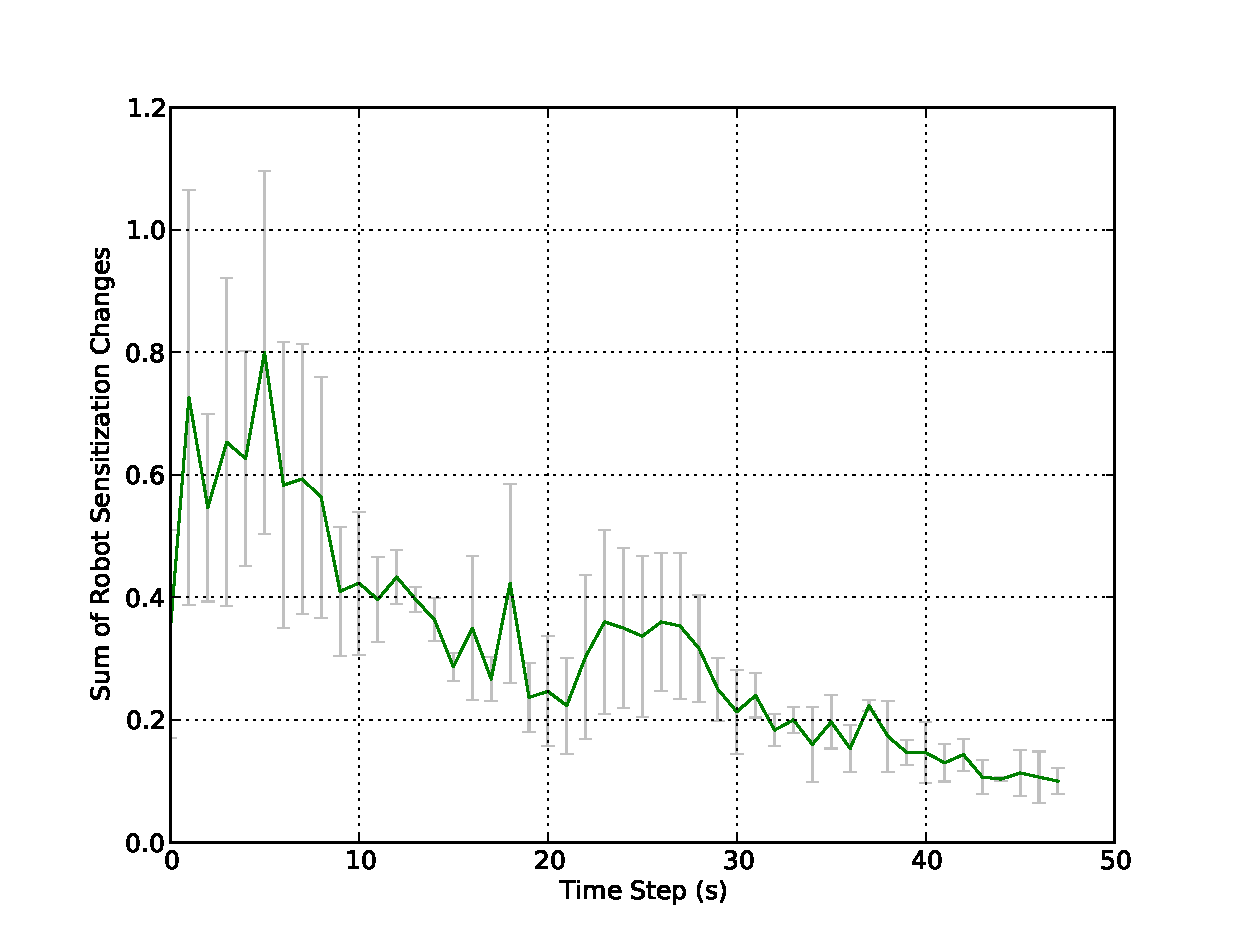
\includegraphics[height=4.2cm, angle=0]
{images/RobotSensitizationStat-Total-50steps.eps}
\caption{\small Changes in sensitizations of all robots}
\label{fig:sensitization-stat} % Give a unique label
\end{minipage}
\end{figure}
%%%%%%%%%%%%%%%%%%%%%%%%%%%%%%%%%%%%%%%%%%%%%%%%%%%%%%%%%%%%%%%%
\section{Conclusions and Future works}
\label{sec:conc}
In this paper we have validated an inter-disciplinary generic model of self-regulated division of labour (DOL) or or multi-robot task allocation (MRTA) by incorporating it in our multi-robot system (MRS) that has emulated a virtual manufacturing shop-floor activities. A centralized communication system has been instantiated to realize this model. We have evaluated various aspects of this model, such as ability to meet dynamic task demands, individual task specializations, communication loads and flexibility in concurrent task completions. A set of metrics has been proposed to observe the DOL in this system. From our experimental results, we have found that AFM can meet the requirements of dynamic DOL by the virtue of its self-regulatory behaviours. Our centralised communication system broadcasts information to all the robots from a central server. This has the advantage of minimising the communication load and the disadvantage of a single point of failure. In the future, we will explore local peer-to-peer communication models in a MRS having about 40 E-puck robots.
%%
\bigskip
\subsubsection*{Acknowledgements. } 
This research has been funded by the Engineering and Physical Sciences Research Council (EPSRC), UK, grant reference EP/E061915/1.
%\begin{acknowledgements}
%If you'd like to thank anyone, place your comments here
%and remove the percent signs.
%\end{acknowledgements}
% BibTeX users please use one of
\bibliographystyle{spbasic} 
%\bibliographystyle{spmpsci}      
\bibliography{bib-si} % name your BibTeX data base
% Non-BibTeX users please use
%\begin{thebibliography}{}
%\bibitem{Bonabeau+1999}
%Bonabeau, E., Dorigo, M. and Theraulaz, G.:
%Swarm intelligence: from natural to artificial systems.
%Oxford University Press (1999)
%\bibitem{Gerkey+2004}
%Gerkey, B. P. and Mataric M. J.:
%A Formal Analysis and Taxonomy of Task Allocation in Multi-Robot Systems.
%The International Journal of Robotics Research, 23 (2004)
%\bibitem{Parker2008}
%Parker, L. E.:
%Distributed Intelligence: Overview of the Field and its Application in Multi-Robot Systems.
%Journal of Physical Agents, 2, 5-14 (2008)
%\bibitem{Lerman+2006}
%Lerman, K., Jones, C., Galstyan, A. and Mataric, M. J.:
%Analysis of Dynamic Task Allocation in Multi-Robot Systems. 
%The International Journal of Robotics Research, 25, 225 (2006)
%\bibitem{Shen+2001}
%Shen, W., Hao, Q., Yoon, H. and Norrie, D.:
%Applications of agent-based systems in intelligent manufacturing: An updated review. Advanced Engineering Informatics, 20, 415-431, Elsevier (2006)
%\bibitem{Dias+2006}
%Dias, M. B., Zlot, R. M., Kalra, N. and Stentz, A.:
%Market-based multirobot coordination: A survey and analysis. 
%Proceedings of the IEEE, 94, 1257-1270, IEEE (2006)
%\bibitem{Liu+2007} 
%Liu, W., Winfield, A. F. T., Sa, J., Chen, J. and Dou, L.:
%Towards Energy Optimization: Emergent Task Allocation in a Swarm of Foraging Robots. Adaptive Behavior, 94, 1257-1270 (2007)
%\bibitem{Sayer+1992}
%Sayer, A. and Walker, R.: 
%The new social economy : reworking the division of labor.
%Blackwell (1992)
%\bibitem{Kogut2000}
%Kogut, B.: 
%The network as knowledge: generative rules and the emergence of structure. 
%Strategic Management Journal, 21, 405-425 (2000)
%\bibitem{Elsa}
%Arcaute, E.; Christensen, K.; Sendova-Franks, A.; Dahl, T.; Espinosa, A. and Jensen, H. J. : 
%Division of labour in ant colonies in terms of attractive fields. 
%Ecological Complexity, Elsevier (2008)
%% etc
%\bibitem{SwisTrack}
%Lochmatter T., Roduit P., Cianci C., Correll N., Jacot J., and Martinoli A.: 
%SwisTrack - A Flexible Open Source Tracking Software for Multi-Agent Systems. 
%In Proceedings of the IEEE/RSJ 2008 International Conference on Intelligent Robots and Systems (IROS 2008), 4004-4010, IEEE (2008)
%\end{thebibliography}
%
\end{document}
